\section{Tutorial}\label{sec:tutorial}

Before actually using the \app solution on a smartphone, both the \be and a \ter have to be running.
Hence this chapter starts with installation instructions for \be and \ter.

General note: a command line starting with \# indicates a root shell, a \$ symbol indicates one without super-user privileges.

\subsection{Install and Launch Backend Server}

The server was implemented based on the JavaScript (JS) technologies \node and \textit{ME(A)N.js} (M = \mongo, E = $express.js$ [web server], A = $angular.js$ [currently not used], N = \node).
Hence it requires a running \mongo database and \node to be installed.
This chapter serves as a recommendation for starting the server.
Experienced users may also install some components locally (without the $-g$ option) or omit some parts.\medskip\\
1.) Install \node.\smallskip\\
2.) Install $npm$, the Node Package Manager.\smallskip\\
3.) Download \mongo.\smallskip\\
4.) Start \mongo via
\begin{lstlisting}
   $ <path-to-mongodb>/bin/mongod
\end{lstlisting}
5.) Install $bower$, a package manager.
\begin{lstlisting}
   # npm install -g bower
\end{lstlisting}
6.) Install $grunt$, a JS task runner for automation.
\begin{lstlisting}
   # npm install -g grunt-cli
\end{lstlisting}
7.) Install $vows$, a JS framework for writing and executing test suites. This is only necessary if tests need to be run.
\begin{lstlisting}
   # npm install -g vows
\end{lstlisting}
8.) Install all \node dependencies of the \be server. $npm$ automatically loads all dependencies defined in $package.json$ and stores them locally.
\begin{lstlisting}
   $ npm install
\end{lstlisting}
9.) Finally, \textbf{run the server} via the $grunt$ client (optionally with the environment variable \textit{NODE\_ENV=test}).
\begin{lstlisting}
   $ grunt
\end{lstlisting}\bigskip
(10.) Optionally, run the $vows$ test suite (change to $/test$ directory first; \textit{NODE\_ENV=test} is required for some unit tests).
\begin{lstlisting}
   $ vows interfaces-test.js --spec
\end{lstlisting}

\subsection{Install and Launch NFC Terminal}
Install the necessary components by issuing the following command on a Raspberry Pi with Raspbian (Debian Wheezy):
\begin{lstlisting}[breaklines=true]
   # apt-get install libusb-dev build-essential autoconf2.64 libtool python3 gettext libreadline-dev
\end{lstlisting}
%
First, install libnfc in the following manner:
\begin{lstlisting}[breaklines=true]
   $ cd ~
   $ git clone https://github.com/nfc-tools/libnfc.git
   $ cd libnfc
   $ # Compilation
   $ autoreconf -vis
   $ ./configure --sysconfdir=/etc --with-drivers=pn532_spi
   $ make
   # make install
\end{lstlisting}
Copy the sample configuration file to the system location:
\begin{lstlisting}[breaklines=true]
   # mkdir /etc/nfc
   # cp libnfc.conf.sample /etc/nfc/libnfc.conf
\end{lstlisting}


%
Edit the content of the configuration file. The relevant lines should be configured as follows:
\begin{lstlisting}[breaklines=true]
allow_autoscan = true
log_level = 2
device.name = "itead_pn532"
device.connstring = "pn532_spi:/dev/spidev0.0:500000"
\end{lstlisting}
%
Install pyNFC (\url{https://github.com/grandcat/pynfc}) for Python 3 as described in its \texttt{README.md}.
Open terminal and change into the cloned directory.
\begin{lstlisting}
cd ~/tum_getin/code/nfcTerminal/PyNfcTerminal
\end{lstlisting}
Execute the main.py:
\begin{lstlisting}
python3 main.py
\end{lstlisting}


%cd ~git d
%git clone https://github.com/grandcat/tum_getin.git
%
%sudo apt-get install python3-crypto
%
%libnfc:
%wget https://libnfc.googlecode.com/files/libnfc-1.7.0.tar.bz2
%tar -jxvf libnfc-1.7.0.tar.bz2
%cd libnfc-1.7.0 
%./configure --prefix=/usr --sysconfdir=/etc --with-drivers=pn532_uart,pn532_spi,pn532_i2c 
%make install all 
%
%git clone https://github.com/ikelos/pynfc.git
%cd pynfc/src	
%2to3 -w nfc.py
%
%mv nfc.py ~/tum_getin/code/nfcTerminal/PyNfcTerminal
%cd ~/tum_getin/code/nfcTerminal/PyNfcTerminal
%
%python3 main.py



\subsection{Use the GetInTUM Android Application}

To use the GetInTum application, the backend server address needs to be adjusted in the fragments and the activities.
The workflow for the user is descibed as followed.  

\begin{table}[ht]
\caption{App user workflow description}
\centering
\begin{tabular}{*{2}{m{0.48\textwidth}}}
\hline
On the first app start, this is the page
that is displayed. The user has to enter his TUM-ID (e.g ga00aaa).
He gets feedback if his ID is valid as soon as he clicks the $Send$ Button
&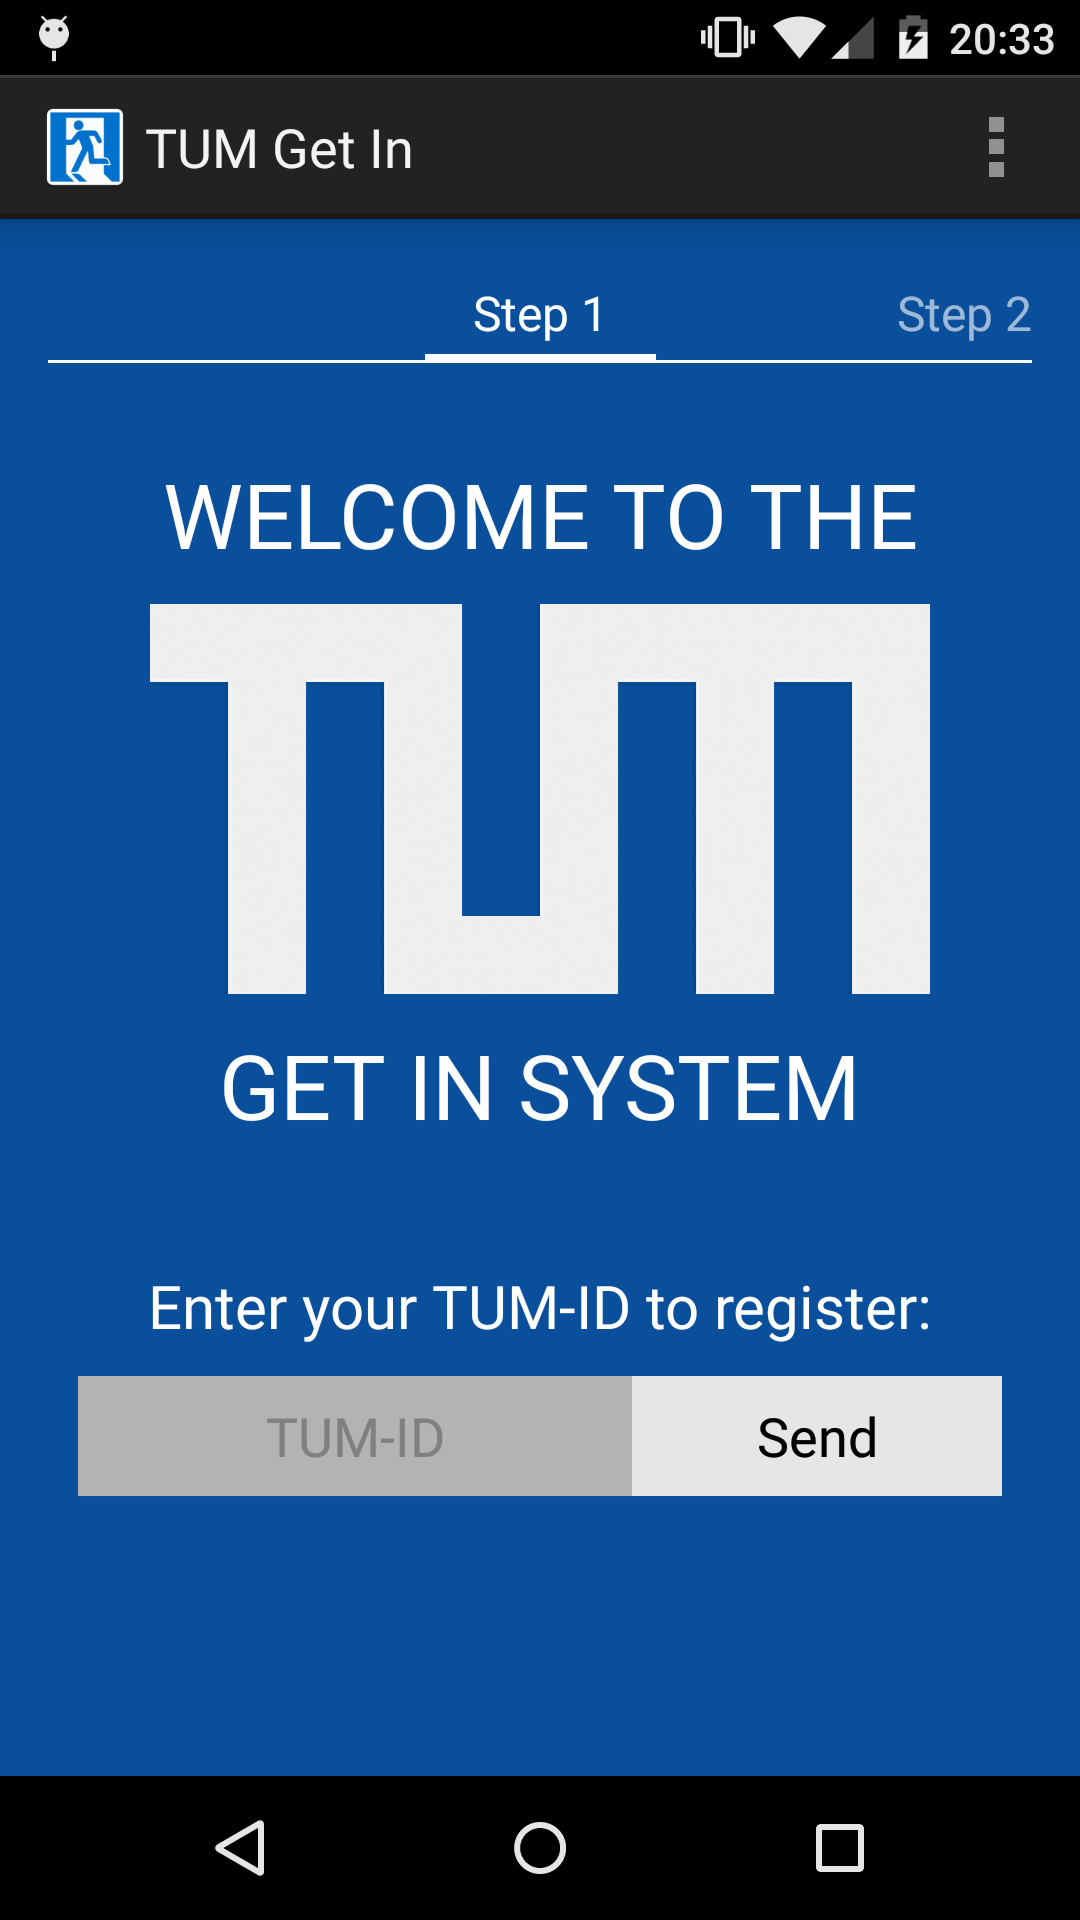
\includegraphics[scale=0.1]{RegisterStep1}\\
\hline
If the entered ID is valid, the backend answers with a created token for
the user which is listed in the private user TUMOnline account.
The user can open the TUMOnline site directly with a click on the button.
Additionally, the status of the token activation can be updated. On an app restart or resume, the status will also be checked and the user will be forwarded to the next page.
&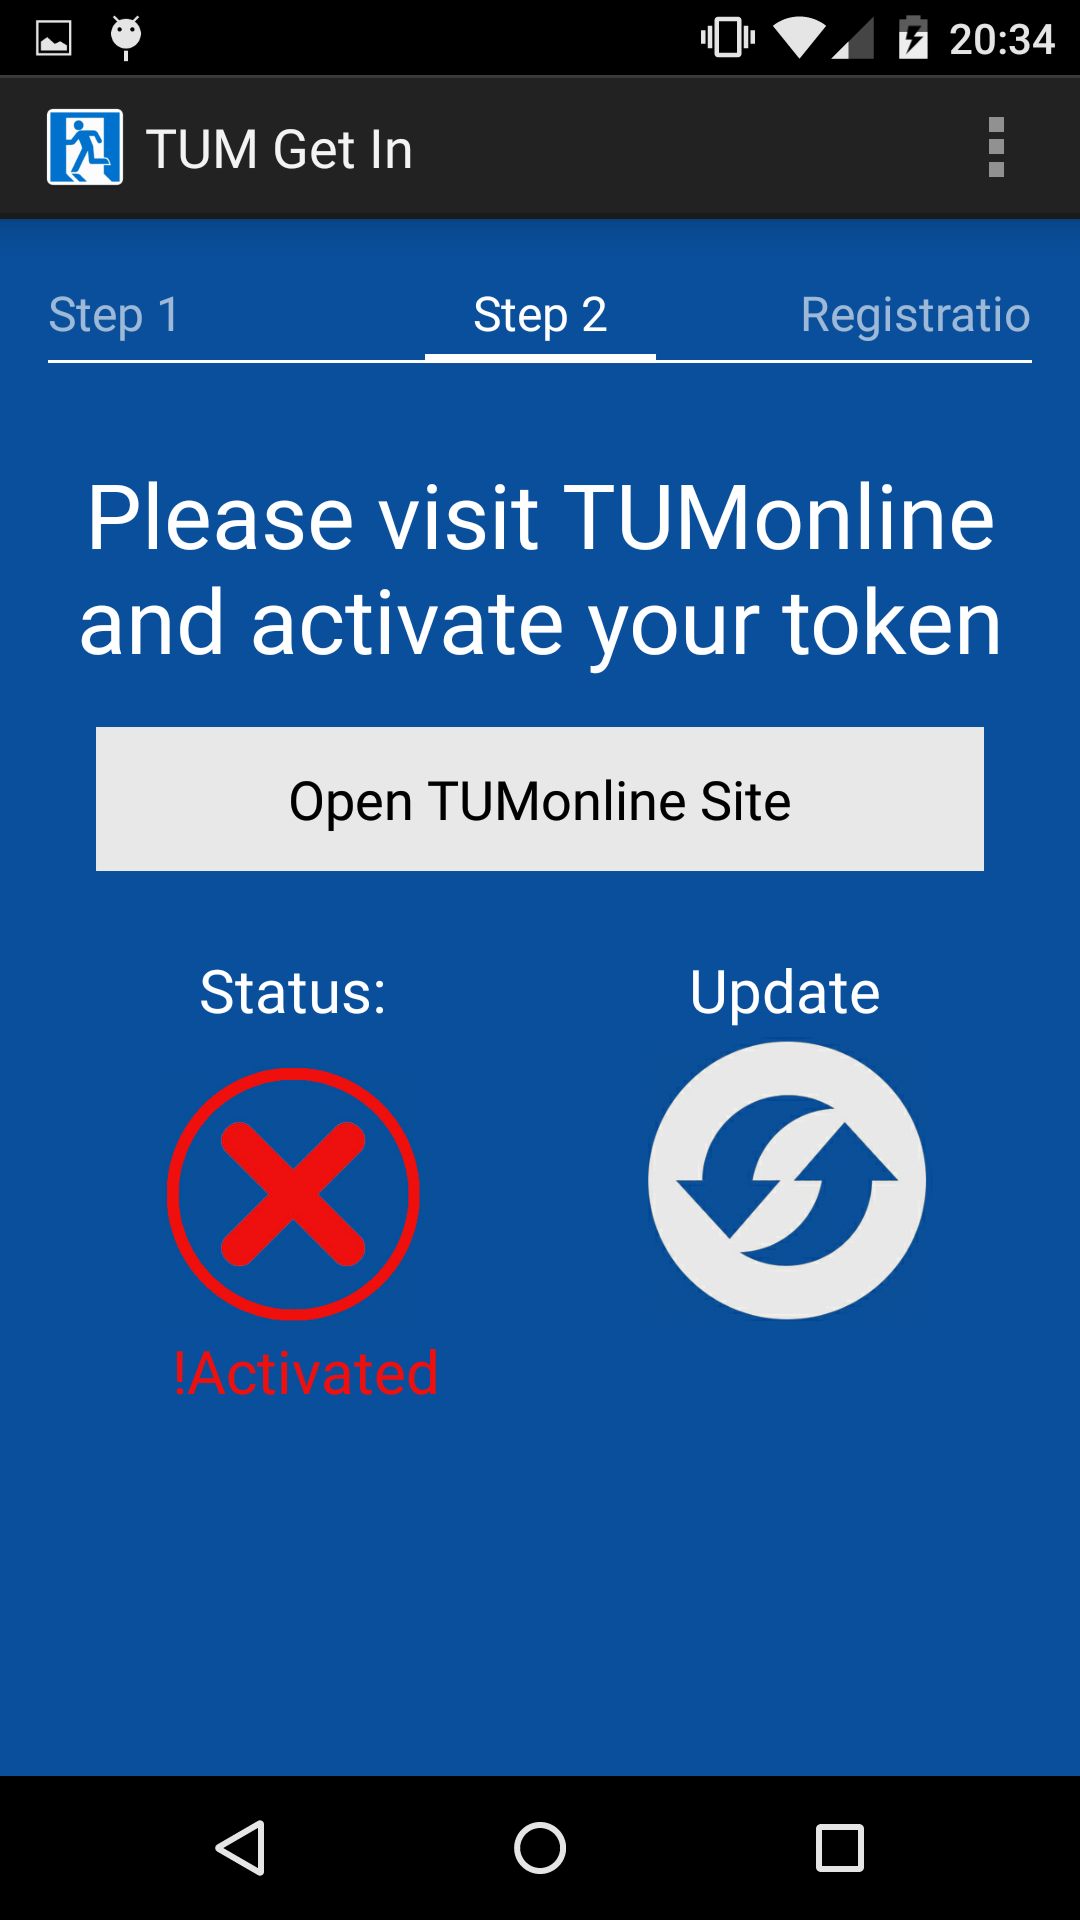
\includegraphics[scale=0.1]{RegisterStep2_not_Activated}\\
\hline
If the registration is completed, the user will see the last page of the registration process.
In case of swiping through the pages that are not completed, an appropriate status will be displayed. On a button click, the ProgressActivity will be shown.
An explicit app start is not needed to use the door NFC terminals. The app will start the
ProgressActivity by itself, informing the user about the communication process
&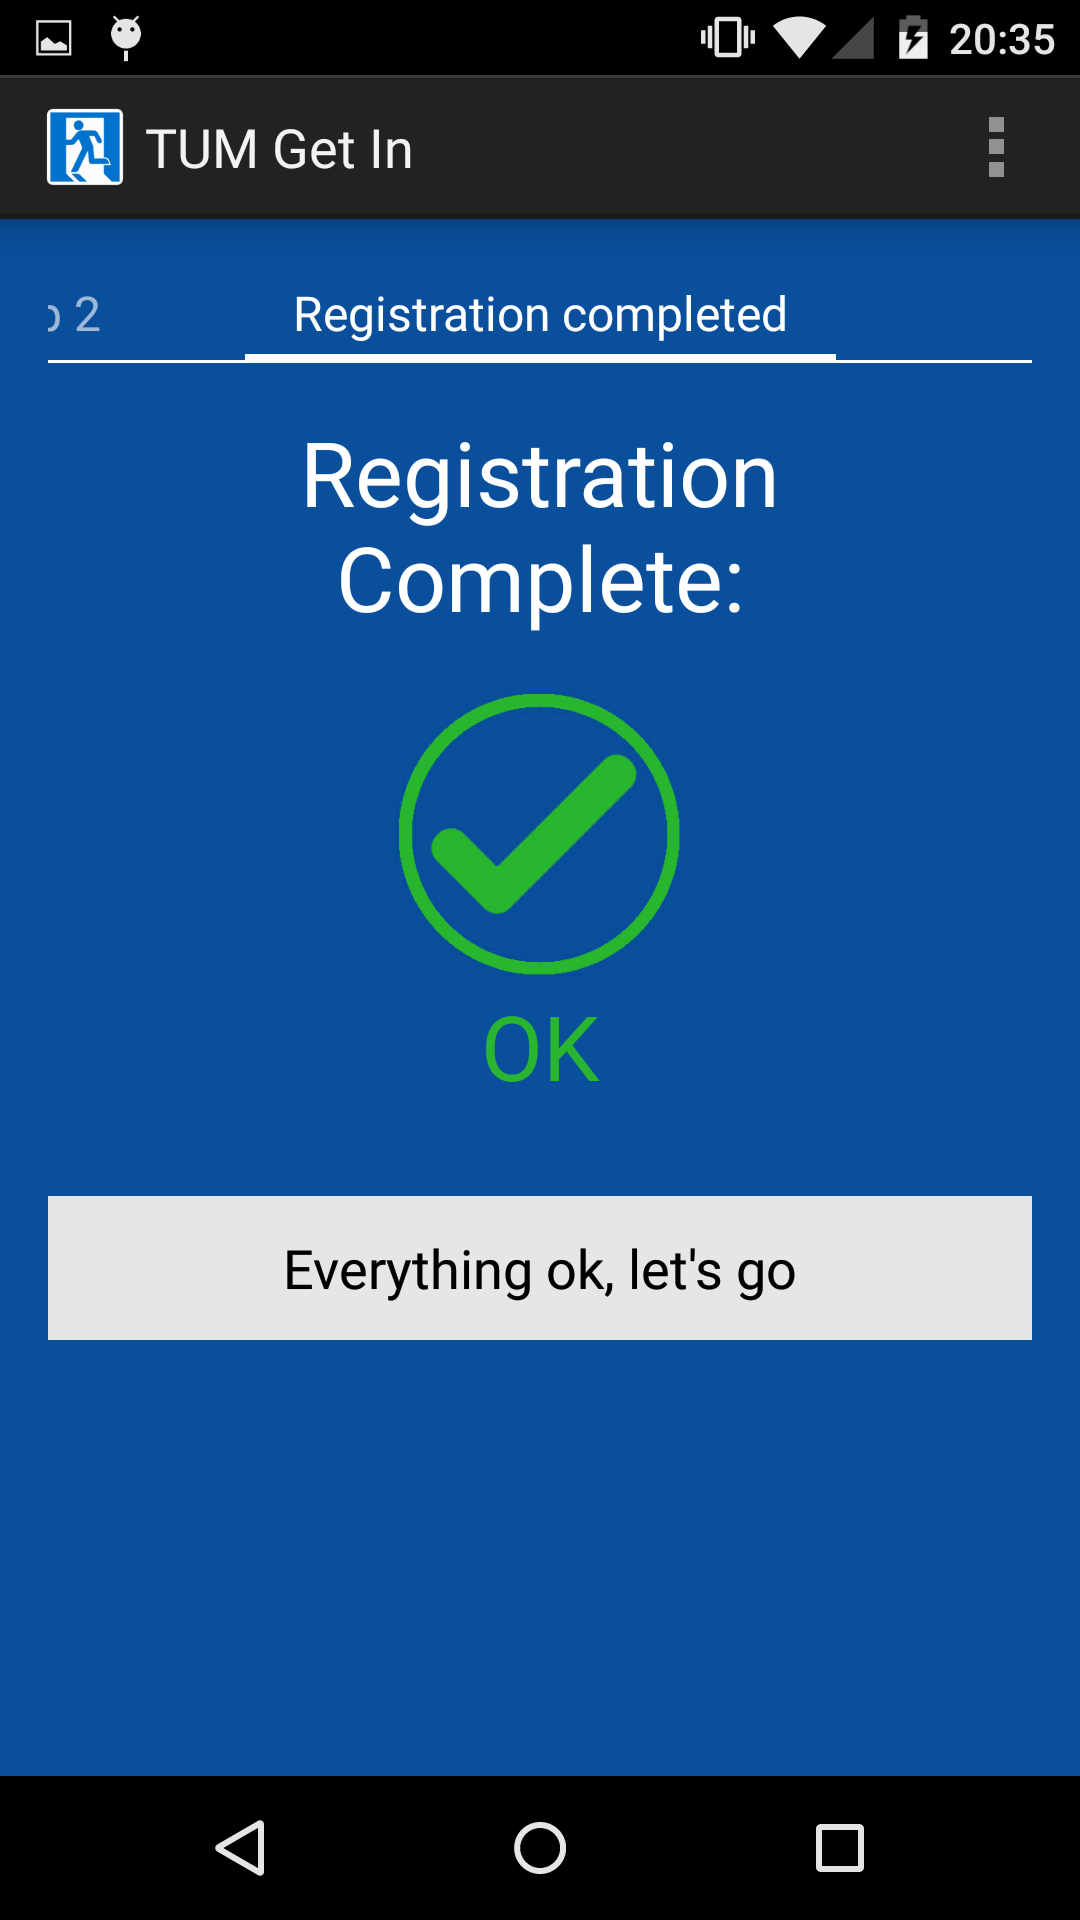
\includegraphics[scale=0.1]{RegisterStep3_Registered}\\

\end{tabular}
\label{tab:gt}
\end{table}

